\section{Introduction}
For this assignment, we analyzed the Jeffrey Epstein document corpus as a multilayer network using graph analytics techniques. The released documents provide a unique opportunity to examine how social access, mobility, money, and institutional influence interacted within a highly interconnected ecosystem.
We structured the analysis in two main stages. First, we examined documented co-travel relationships and shared locations to understand how movement and physical proximity connected elite social circles. We then focused on the financial infrastructure of the network, including settlements, donations, operational funding, and political or institutional relationships.
Finally, we combined both layers to explore how mobility and money reinforced one another structurally. Together, these analyses provide a clearer picture of how brokerage, influence, and coordination emerged within the documented Epstein network.
Importantly, the findings in this assignment describe patterns within an LLM-extracted graph derived from released documents, rather than definitive historical or legal conclusions.
\section{Data and methodology}
The analysis is based on a graph database generated from the publicly released Jeffrey Epstein documents made available by the U.S. House Oversight Committee between 2024 and 2025. The dataset includes a wide variety of materials, such as flight logs, financial records, legal filings, depositions, internal communications, schedules, and investigative documents.
\subsection{Large language model}
To make this large and unstructured corpus analyzable, the open-source Epstein-doc-explorer project used a Large Language Model (LLM) to extract structured relationships from the documents. These extracted relationships were then stored inside a graph database containing more than 546,000 nodes and approximately 1.4 million edges.
The graph primarily consists of four main components:
\begin{itemize}
    \item \textbf{Entities:} people and organizations referenced in the documents
    \item \textbf{Claims:} subject--action--object relationships extracted from text
    \item \textbf{Documents:} the original source material from which claims were extracted
    \item \textbf{Locations:} geographic places connected to claims and entities
\end{itemize}
These components are connected through relationships such as \texttt{RELATED\_TO}, which links entities through extracted actions, and \texttt{AT\_LOCATION}, which connects claims to geographic locations.
\subsection{Subgraphs}
For this assignment, we focused only on the relationships most relevant to our research questions. Since a large portion of the graph consisted of AI-generated metadata and semantic tagging, we filtered the dataset down to the extracted relational structure itself.
From this filtered graph, we constructed three focused subgraphs and a comprehensive scatterplot:
\begin{itemize}
    \item A co-travel network, based on actions such as ``flew with,'' ``flew on,'' and ``traveled with''
    \item A bipartite person-location network, connecting individuals to locations where they were documented to appear
    \item A financial transaction network, based on actions related to payments, donations, transfers, loans, and settlements
    \item A multilayer brokerage analysis, assessing the existence of an overlap in social-travel and financial networks based on documented activity
\end{itemize}
This reduction process lets us isolate the structural backbone of the social and financial dimensions of the network, minimizing semantic noise from unrelated metadata.
\subsubsection{Co-travel network}
The co-travel network allows us to identify which individuals were actively and physically involved in the network's operations. The frequency of co-travel, especially regarding flights to and from Little Saint James, provides a strong indicator of physical proximity to the core crimes. Individuals who flew repeatedly with Epstein to his private island are structurally distinct from those whose involvement remained peripheral.
Beyond individual frequency, we can also examine the community structure of the co-travel network and identify the brokers who bridge between those communities. Under Burt's structural-holes framework, the analytically interesting positions are not the densest local clusters but the individuals who sit between them, since their removal would fragment the network into disconnected sub-circles. Identifying these brokers is therefore central to characterising how Epstein's documented travel network was organised, and how distinct sub-circles were connected through a small number of high-betweenness individuals.
\subsubsection{Person-location network}
The person-location network complements this by assessing the qualitative character of an individual's presence. We can differentiate between people whose footprint was confined to public or commercial venues and those who entered the restricted, private spaces that functioned as the operational core. Documented presence in these private locations carries a completely different evidentiary weight than a footprint in purely institutional or public settings.
\subsubsection{Financial network}
Finally, the financial network is designed to surface actors who were deeply involved in organizing and funding the network, yet avoided any personal physical presence. By following the money, we aim to reconstruct how the crimes were financed, how victims were silenced through settlements, and which institutions were used to buy legitimacy. Together, combining these three analytical layers allows us to propose a clear typology of involvement across the network:
\begin{itemize}
    \item Suspicious physical participants in operational spaces,
    \item Individuals who are financially implicated but lack a physical footprint in core locations, and
    \item Peripheral actors whose involvement remains ambiguous based on the current evidence.
\end{itemize}
\subsubsection{The multilayer brokerage analysis}
The multilayer analysis allows us to compare an individual's position across two structurally independent dimensions of the documented record: the co-travel network and the financial-transaction network. The central question is whether the same individuals are prominent in both layers, or whether each layer surfaces a distinct cast of actors. An individual documented in co-travel but not in transactions reflects a relationship that was social or logistical in nature rather than financial; conversely, an individual documented in transactions but not in co-travel reflects an institutional, advisory, or business relationship conducted without personal travel. The individuals documented in both layers are of particular interest: their connection to Epstein traverses multiple modalities of contact, making them the most multi-modally entangled actors in the corpus.
\subsection{Extraction methodology and limitations}
The graph used in this assignment is not a direct copy of the original documents, but a derived network generated through LLM-based extraction. As a result, several limitations must be considered throughout the analysis.
First, entity recognition is imperfect. The same individual may appear under multiple names or titles. For example, ``Bill Clinton'' and ``President Clinton'' can exist as separate entity nodes even though they refer to the same person. During the analysis, we identified several duplicate clusters. To reduce this issue, the most important duplicates were manually merged through a canonicalization process.
Second, the action labels inside the \texttt{RELATED\_TO} relationships are not standardized. Similar interactions can appear under different formulations such as ``flew with,'' ``flew on,'' ``traveled with,'' or ``boarded with.'' Constructing the co-travel network therefore required carefully selecting and filtering the relevant action labels before analysis.
Finally, and most importantly, the graph reflects what the LLM extracted from the released documents rather than a complete reconstruction of historical reality. A relationship in the graph only indicates that the model identified such a connection within the document corpus. Likewise, the absence of a relationship does not prove that an event never occurred. Some extracted relationships may also be incomplete or overly generalized due to ambiguity in the source material.
Consequently, all findings in this assignment should be interpreted as observations about the extracted graph structure rather than definitive factual or legal conclusions.
\section{Exploration of the co-travel and bipartite person-location network}
\subsection{Action vocabulary inventory}
Before any filter is committed, the actual action strings on flight-related \texttt{RELATED\_TO} edges must be inventoried. We checked how many contain ‘flew’, ‘flight’, ‘travel, ‘board’,  ‘plane’  with \texttt{count(*)} AS n and we get as return our following top entries.
\begin{table}[H]
    \centering
    \begin{tabular}{l c l}
        \toprule
        Action & Count & Interpretation \\
        \midrule
            traveled to & 299 & Directional destination, not co-travel \\
            traveled with & 99 & Strong co-travel signal, mode-ambiguous \\
            planned travel to & 49 & Intent, not actual presence \\
            flew & 38 & Directional, often "flew to" \\
            flew with & 30 & Strongest co-travel signal \\
            flew on & 25 & Shared aircraft signal \\
            serves on board of & 22 & False positive — refers to corporate boards \\
            served on board of & 21 & Same false positive \\
        \bottomrule
    \end{tabular}
    \caption{Selected actions from the flight-vocabulary inventory.}
    \label{tab:flight_vocabulary}
\end{table}
\subsection{Filtering}
\subsubsection{Flight co-travel network}
The flight subgraph filters \texttt{RELATED\_TO} edges by the committed action vocabulary and excludes any endpoint that the LLM extracted as an aircraft, airline, or known location (which the LLM occasionally typed as Entity rather than Location). Which we did with \texttt{toLower(r.action) IN ['flew with', 'flew on', 'traveled with']} The filter is symmetric (both endpoints must be person-like) and case-insensitive.
\subsubsection{Bipartite person-location network}
The flight subgraph captures the social co-travel layer but says nothing about where people were. To add the geographic dimension, a second subgraph is constructed: a bipartite graph in which Entity nodes are connected to Location nodes by a derived edge type \texttt{VISITED}, where the weight of an edge equals the number of distinct claims in which the entity and location co-occur.
\subsection{Entity and location canonicalisation}
LLM-based extraction produces entity-resolution duplicates. Verification queries identified these clusters in the flight-network entity set:
\begin{table}[H]
    \centering
    \begin{tabular}{l c c}
        \toprule
        Canonical Location & Number of Variants Merged & Post-merge Weighted Degree \\
        \midrule
            Palm Beach & 18 (incl. Epstein's mansion variants) & 2195 \\
            New York City & 5 & 1833 \\
            Mar-a-Lago & 5 & 144 \\
            Washington, D.C. & 3 & 129 \\
            Little Saint James & 7 & 116 \\
            U.S. Virgin Islands & 6 & 105 \\
        \bottomrule
    \end{tabular}
    \caption{Canonical location clusters after merging LLM-extracted variants.}
    \label{tab:canonical_locations}
\end{table}
The Palm Beach cluster is the most aggressive merge: it folds the specific address "358 El Brillo Way, Palm Beach" (Epstein's actual Palm Beach mansion) into the broader "Palm Beach" canonical, along with all West Palm Beach and Palm Beach County variants. This loses some specificity as visiting the Town of Palm Beach is innocent in many contexts, while specifically visiting 358 El Brillo Way is not but produces a cleaner bipartite figure. We are aware of the tradeoff with merging  ``358 El Brillo Way'' with ``Palm Beach'' but given the names and derivations of ``358 El Brillo Way'' were so sparse the positives outweigh the negative. We do however still hold this into account in our interpretation.
\section{Analysis I: the flight co-travel network}
The filtered flight subgraph, restricted to its giant connected component, contains approximately 80 nodes and 61 edges. The full graph statistics computed in Gephi:
\begin{table}[H]
    \centering
    \begin{tabular}{l c l}
        \toprule
        Metric & Value & Interpretation \\
        \midrule
            Nodes  & \textasciitilde{}80 & Personnel in the documented co-travel set \\
            Edges  & 61 & Distinct co-travel relationships \\
            Average degree & 1.205 & Sparse, hub-dominated \\
            Network diameter & 4 & Tight network \\
            Average path length & 2.452 & Most pairs within 2--3 hops \\
            Modularity  & 0.344 & Moderate community structure \\
        \bottomrule
    \end{tabular}
    \caption{Structural metrics of the flight co-travel subgraph.}
    \label{tab:flight_metrics}
\end{table}
The average degree of 1.205 indicates an extremely sparse graph. Almost every node has only one to two connections; the network is dominated by a small number of hubs. This is structurally consistent with Burt's structural-holes story, Epstein's documented value as a connector derived from bridging otherwise-disconnected actors, not from belonging to a dense pre-existing community.
We then also computed betweenness centrality on the giant component and a visualization of the found top-five entities:
\begin{table}[H]
    \centering
    \begin{tabular}{c l c c l}
        \toprule
        Rank & Entity & Betweenness & Degree & Interpretation \\
        \midrule
            1 & Jeffrey Epstein & 411.5 & 12 & Central hub, as expected \\
            2 & Bill Clinton & 266.5 & 6 & Secondary broker \textasciitilde{}65\% of Epstein \\
            3 & Unknown Person A & 80.0 & 3 & Anonymised entity bridging sub-circles \\
            4 & Alan M. Dershowitz & 48.0 & 4 & Tertiary broker (legal-counsel role) \\
            5 & Lawrence Summers & 12.0 & 3 & Lower-tier bridge \\
        \bottomrule
    \end{tabular}
    \caption{Top entities by betweenness centrality in the flight co-travel subgraph.}
    \label{tab:flight_betweenness}
\end{table}

\begin{figure}[H]
    \centering
    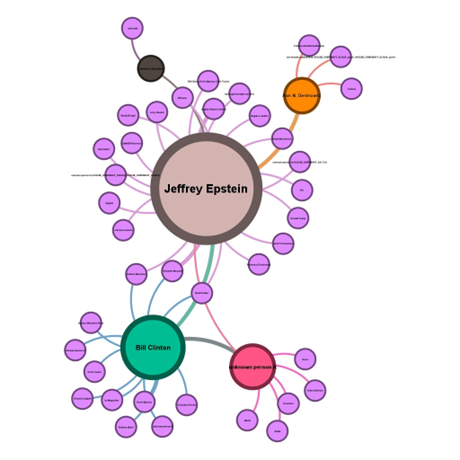
\includegraphics[width=0.9\textwidth]{figures/4.1 Co flights.png}
    \caption{Flight co-travel network. Nodes are individuals; edges are documented "flew with / flew on / traveled with" claims. Node size is proportional to betweenness centrality. Node colour is proportional to Louvain community assignment. Generated in Gephi using ForceAtlas 2 layout.}
    \label{fig:flight_co_travel}
\end{figure}
Three observations from this network deserve particular attention.
First, Bill Clinton’s position in the network is not simply that of a frequent traveler, but that of a structural broker. Despite having fewer direct connections than Epstein, his betweenness centrality remains exceptionally high, meaning that several individuals connect to the broader network primarily through him. Structurally, Clinton appears as a secondary bridge between otherwise separated groups.
Second, the appearance of ``Unknown Person A'' as one of the strongest brokers is methodologically significant. At first glance one might think that this is a single person kept secret that has a lot of involvement with Jeffrey Epstein. In reality this is not just one person but a whole lot of different people across different documents that stay anonymous, for example victims of Jeffrey Epstein. It makes sense that this has a high betweenness as the victims range across a lot of different documents and involve a lot of different people.
Third, the co-travel graph is highly brokered rather than densely interconnected. Most individuals are linked through a small number of central intermediaries instead of belonging to tightly connected communities. This suggests a network built around connecting separate elite social circles rather than maintaining one cohesive group.
\section{Analysis II: bipartite person-location network}
The bipartite network was constructed by deriving a \texttt{VISITED} edge from each flight-network entity to each Location node at which the entity is documented to have appeared, weighted by the number of distinct claims. After applying the location canonicalization, the working graph contains 225 nodes (a mix of Entity and Location), 119 \texttt{VISITED} edges, and is naturally bipartite (Entity nodes connect only to Location nodes and vice versa).
Statistical analysis was performed in Gephi using the same pipeline as for the flight subgraph. The key metrics:
\begin{table}[H]
    \centering
    \begin{tabular}{l c}
        \toprule
        Metric & Value \\
        \midrule
            Total nodes & 225 \\
            Edges (VISITED) & 119 \\
            Network diameter & 4 \\
            Average path length & 2.285 \\
            Modularity (Louvain) & 0.319 \\
        \bottomrule
    \end{tabular}
    \caption{Structural metrics of the bipartite person-location subgraph.}
    \label{tab:bipartite_metrics}
\end{table}
\subsection{Centrality ranking: entities}
In the bipartite network, betweenness centrality measures whether a node's removal would disconnect parts of the entity-location structure.
\begin{table}[H]
    \centering
    \begin{tabular}{c l c c}
        \toprule
        Rank & Entity & Betweenness & Weighted Degree \\
        \midrule
            1 & Unknown Person A & 4099.27 & 1200 \\
            2 & Jeffrey Epstein & 3743.92 & 3990 \\
            3 & Donald Trump & 514.23 & 735 \\
            4 & Alan M. Dershowitz & 437.16 & 317 \\
            5 & Unknown Person B & 411.78 & 155 \\
            6 & Ehud Barak & 341.20 & 406 \\
            7 & Virginia Roberts Giuffre & 306.60 & 235 \\
            8 & Bill Clinton & 293.65 & 224 \\
            9 & Ghislaine Maxwell & 148.26 & 345 \\
            10 & Steve Bannon & 107.23 & 126 \\
        \bottomrule
    \end{tabular}
    \caption{Top entities by betweenness centrality in the bipartite network.}
    \label{tab:bipartite_entities}
\end{table}
Three observations on the entity rankings. First, "unknown person A" surpasses Epstein himself in betweenness here, even though Epstein has more than three times the weighted degree. This is because the anonymised entity bridges across more distinct location clusters per edge than Epstein does, whose connections concentrate around a smaller set of high-weight personal locations. Second, the ranking now picks up figures who were not prominent in the flight subgraph, notably Ehud Barak (former Israeli Prime Minister) and Steve Bannon, both of whom have documented presence at multiple locations in the corpus without appearing prominently in flight-action claims. Third, Donald Trump now appears at rank 3, well above his position in the flight subgraph, because his location footprint is broader and more cross-cutting (Mar-a-Lago, Palm Beach, White House, Washington DC, Camp David, Andrews Air Force Base, Oval Office, plus several international destinations).

\subsection{Centrality ranking: locations}
\begin{table}[H]
    \centering
    \begin{tabular}{c l c c}
        \toprule
        Rank & Location & Betweenness & Weighted Degree \\
        \midrule
            1 & New York City & 660.72 & 1823 \\
            2 & Palm Beach & 598.58 & 2195 \\
            3 & Camp David & 203.61 & 161 \\
            4 & London & 144.69 & 186 \\
            5 & White House & 89.36 & 264 \\
            6 & Washington, D.C. & 85.41 & 129 \\
            7 & Little Saint James & 56.54 & 116 \\
            8 & U.S. Virgin Islands & 45.22 & 105 \\
            9 & Mar-a-Lago & 33.03 & 144 \\
        \bottomrule
    \end{tabular}
    \caption{Top locations by betweenness centrality in the bipartite network.}
    \label{tab:bipartite_locations}
\end{table}
New York City and Palm Beach are the two highest-betweenness locations. Their analytical role is as "social glue" places shared across otherwise-distinct social circles, with high visitor diversity. Camp David is surprisingly third; its position is driven by being a destination shared between Trump-cluster figures and several other government-official entities in the corpus, making it a small but structurally pivotal bridge between subgraphs that would otherwise be more separable.
Notably, the high-weighted-degree private destinations. Palm Beach (2,195), Little Saint James (116), Mar-a-Lago (144) do not all map onto high betweenness. Palm Beach has both, but Mar-a-Lago and Little Saint James are relatively low-betweenness despite their substantive importance. The interpretation is that these locations sit within a tightly connected sub-cluster rather than bridging across the wider network, they are "core" locations rather than "bridge" locations.
\subsection{Asymmetric private-location footprints}
One of the most striking findings in the bipartite analysis concerns the differing location footprints of Donald Trump and Bill Clinton. We extracted the graphs just concerning the location nodes of these two people.

\begin{figure}[H]
    \centering
    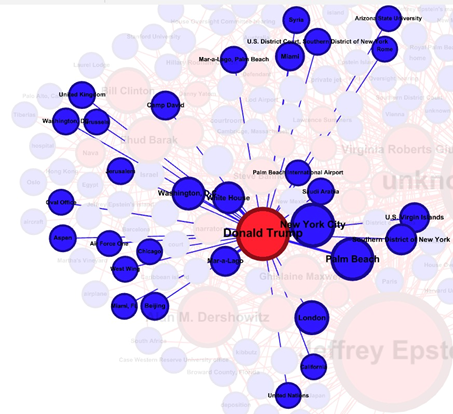
\includegraphics[width=0.8\textwidth]{figures/4.2 Donald Trump.png}
    \caption{Donald Trump location network}
    \label{fig:trump_locations}
\end{figure}

As we can see in our figure, Trump’s documented locations in the LLM-extracted graph include Mar-a-Lago, the White House, Camp David, Washington D.C., New York City, Palm Beach, and several international destinations. While he does appear connected to the broader ``U.S. Virgin Islands'' node, the graph contains no extracted claims linking him directly to the specific ``Little Saint James'' location node.

\begin{figure}[H]
    \centering
    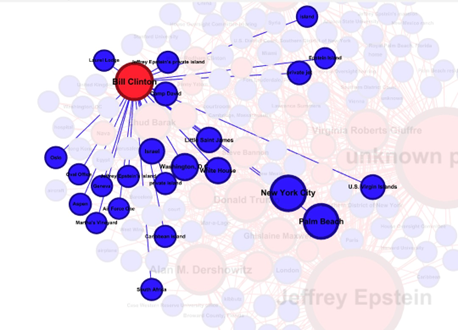
\includegraphics[width=0.8\textwidth]{figures/4.3 Bill Clinton.png}
    \caption{Bill Clinton location network}
    \label{fig:clinton_locations}
\end{figure}
By contrast, the canonical Little Saint James node includes documented connections to figures such as Bill Clinton, Prince Andrew, Virginia Roberts Giuffre, and Ghislaine Maxwell. Clinton’s presence at Little Saint James appears across multiple extracted claims merged during the canonicalization process. As an extra visualization we provide the graph of the Little Saint James network.

\begin{figure}[H]
    \centering
    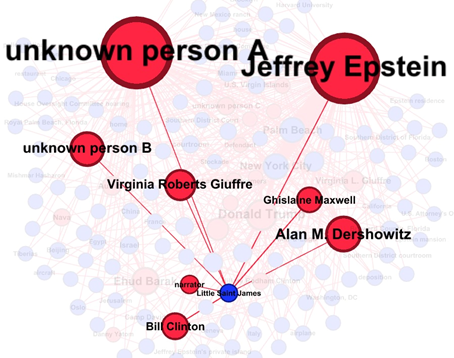
\includegraphics[width=0.8\textwidth]{figures/4.4 Little Saint James.png}
    \caption{Little Saint James network}
    \label{fig:lsj_network}
\end{figure}
Importantly, this does not prove absence or presence in historical reality. The corpus may be incomplete, and LLM extraction itself is imperfect. Nevertheless, the asymmetry between the documented location footprints of Trump and Clinton remains structurally significant and illustrates the type of distinction that multilayer network analysis can reveal.
\section{Analysis III: financial infrastructure}
\subsection{Data}
Although only a small portion of the extracted relationships involve direct financial activity, these transactions form one of the most structurally important layers of the network. Most relationships in the corpus concern communication, meetings, travel, or logistical coordination, while the financial layer reveals how parts of the network were operationally sustained.
To isolate the structural backbone of this financial system, we applied a weight threshold WHERE \texttt{aantal > 4} that retained only entity pairs connected through at least five separate financial interactions. This filtering step removed incidental or one-off transactions and highlighted the recurring financial relationships that formed the core infrastructure.
We then identified financial flows, group them by unique sender--receiver pairs, and generate aggregated \texttt{[g:GELDSTROOM]} relationships in which with SET \texttt{g.transacties = aantal} the number of transactions is stored as a numerical weight property. This weight is later used to determine edge thickness in the network visualization.
\subsection{Settlements, compensation, and legal containment}
We then can use this to extract our betweenness table and a resulting graph revealing several recurring categories of financial activity.
\begin{table}[H]
    \centering
    \begin{tabular}{c l c}
        \toprule
        Rank & Person & Betweenness \\
        \midrule
            1 & Jeffrey Epstein & 1130.5 \\
            2 & Unknown Person A & 264.83 \\
            3 & Bill Clinton & 112 \\
            4 & SEC & 100 \\
            5 & Robert Matthews & 51 \\
            6 & Unknown Person B & 16.83 \\
            7 & Ghislaine Maxwell & 10.3 \\
            8 & Donald Trump & 6.5 \\
            9 & Alan M. Dershowitz & 2.83 \\
        \bottomrule
    \end{tabular}
    \caption{Top people by betweenness centrality in the financial network.}
    \label{tab:financial_betweenness}
\end{table}

\begin{figure}[H]
    \centering
    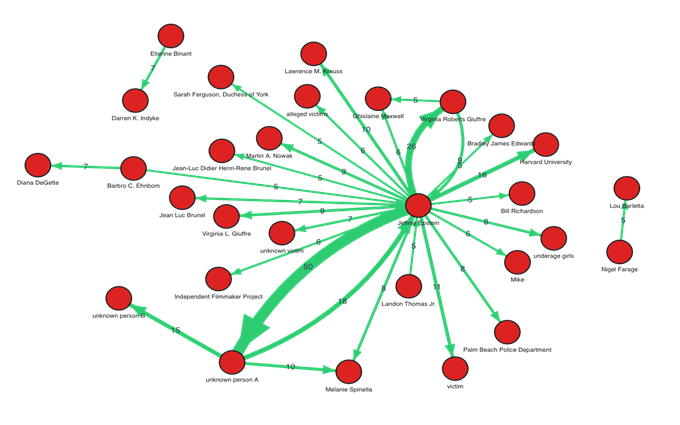
\includegraphics[width=0.9\textwidth]{figures/4.5 Financial activity.png}
    \caption{Graph with recurring categories of financial activity}
    \label{fig:financial_activity}
\end{figure}


One of the clearest patterns in the data involves repeated settlements and compensation-related payments connected to victims, legal representatives, and civil cases. A couple of these are
\begin{itemize}
    \item \textbf{Virginia Roberts Giuffre \& Virginia L. Giuffre (33 transactions total):}
    \item \textbf{Bradley James Edwards (5 transactions):}
    \item \textbf{Anonymous victims (``alleged victims'', ``underage girls'', ``unknown victim'' -- combined $>$30 transactions):}
\end{itemize}
Most of these connections contain operational payments linked to exploitation, to active legal settlement, the silencing of testimony. In the example of Virginia Roberts Giuffre the extracted relationships include operational payments, gifts, medical expenses, and later legal settlements, reflecting a transition from exploitation-related transactions to formal legal resolution
The graph also contains numerous repeated payments involving anonymized or partially redacted victims, including references to ``underage girls,'' ``alleged victims,'' and ``unknown victims.'' These recurring financial relationships suggest that compensation and settlement mechanisms formed a persistent structural component of the broader network rather than isolated incidents.
\subsection{Institutional reputation and philanthropic funding}
A second major category involves donations, research funding, and institutional philanthropy. The financial graph shows repeated funding relationships between Epstein and several academic, scientific, cultural, and institutional actors.
Among the most prominent examples are Harvard University, Lawrence Krauss, and Martin Nowak, all of whom appear repeatedly in donation or research-funding related interactions. These relationships suggest that philanthropy functioned not only as financial activity, but also as a mechanism for acquiring legitimacy, access, and integration into elite intellectual networks.
The graph also contains repeated donation-related interactions involving the Palm Beach Police Department. Structurally, this is particularly notable because Palm Beach represented one of the earliest jurisdictions connected to investigations into Epstein. While the graph alone cannot determine intent, the repeated financial ties illustrate how institutional relationships extended beyond purely social or personal interactions.

\subsection{Operational financing and core associates}
The financial network suggests that the broader system relied heavily on the funding of close operational associates and intermediaries.
\begin{itemize}
    \item \textbf{Jean-Luc Brunel (12 transactions):} Brunel emerged as one of the most financially connected actors in this layer. Beyond references to legal support payments, the graph also contains several high-value transactions, including million-dollar wire transfers and investment-related interactions linked offshore accounts and affiliated companies. Structurally, these repeated financial ties suggest that Brunel functioned as a heavily financed operational partner rather than a peripheral associate.
    \item \textbf{Ghislaine Maxwell (6 transactions):} The extracted claims include loans, legal funding, and other forms of financial support provided by Epstein. Together, these interactions indicate a strong financial dependency relationship as well as coordinated legal and operational activity.
    \item \textbf{Darren Indyke \& Etienne Binant (7 transactions):} This cluster reveals part of the technical banking infrastructure behind the network. The extracted relationships reference wire-transfer systems, banking access, multi-currency transaction capabilities, and transfer limits. Rather than isolated payments, these interactions point toward the operational financial systems that supported international money flows.
\end{itemize}

\subsection{Political influence and strategic networks}
The financial layer also reveals how money was used to build and maintain relationships within political, aristocratic, and elite institutional circles.
\begin{itemize}
    \item \textbf{Sarah Ferguson, Duchess of York (5 transactions):} The graph contains repeated references to loans and debt payments made on her behalf. These interactions illustrate how financial support could reinforce access to high-status social environments and elite circles.
    \item \textbf{Bill Richardson (5 transactions):} The extracted relationships include repeated political donations and financial contributions, reflecting direct engagement with political actors and institutions.
    \item \textbf{Barbro Ehnbom \& Diana DeGette (12 combined transactions):} These interactions highlight the role of fundraising and political coordination within the network. The graph contains references to organizing fundraisers, coordinating political events, and discussing financial contributions involving Epstein, illustrating how financial activity extended into broader political and elite social networks.
\end{itemize}

\section{Analysis IV: multilayer brokerage analysis}
When both layers are combined, the network reveals that mobility and money were not separate systems, but closely interconnected parts of the same structure. The co-travel and location networks show how individuals gained access to one another through shared movement and recurring physical spaces, while the financial network reveals how those relationships were maintained, protected, and operationally supported.
Several locations that emerged as central hubs in the bipartite network, such as Palm Beach, New York City, Mar-a-Lago, and Little Saint James, also appear indirectly connected to major financial relationships. These spaces functioned not only as geographic meeting points, but as environments where social access, institutional influence, and financial coordination overlapped.

\subsection{Cross-layer brokerage analysis}
To compare the social-travel and financial dimensions of the network, documented activity was computed separately for both subgraphs. Each entity was then positioned according to its structural importance in the flight network (x-axis) and the financial network (y-axis). This allows the graph to identify which actors are present across both layers simultaneously.

\begin{figure}[H]
    \centering
    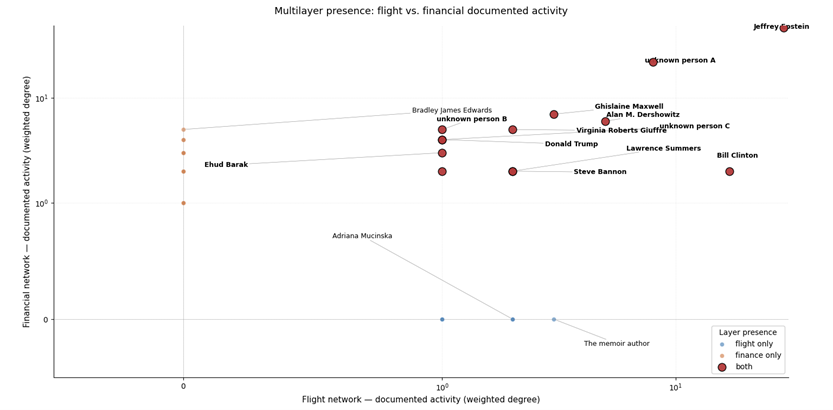
\includegraphics[width=0.9\textwidth]{figures/4.6 multilayer analysis.png}
    \caption{Multilayer brokerage: flight vs. financial structural position}
    \label{fig:multilayer_brokerage}
\end{figure}


Among the 128 entities with positive activity in at least one layer, just over one-tenth (13 entities) are documented across both. The remainder are roughly evenly split between flight-only and finance-only presence.

\subsection{The doubly-active 13}
\begin{table}[H]
    \centering
    \begin{tabular}{l c c}
        \toprule
        Person & Flight Activity (claims) & Financial Activity (claims) \\
        \midrule
            Jeffrey Epstein & 29 & 47 \\
            Unknown Person A & 8 & 22 \\
            Bill Clinton & 17 & 2 \\
            Alan M. Dershowitz & 5 & 6 \\
            Ghislaine Maxwell & 3 & 7 \\
            Virginia Roberts Giuffre & 2 & 5 \\
            Unknown Person B & 1 & 5 \\
            Donald Trump & 1 & 4 \\
            Unknown Person C & 1 & 4 \\
            Lawrence Summers & 2 & 2 \\
            Steve Bannon & 2 & 2 \\
            Ehud Barak & 1 & 3 \\
            Hillary Rodham Clinton & 1 & 2 \\
        \bottomrule
    \end{tabular}
    \caption{The doubly-active 13 entities with documented activity in both networks.}
    \label{tab:doubly_active_13}
\end{table}


The visualization reveals a very small ``doubly-entangled'' core consisting of entities that occupy structurally important positions in both the mobility and financial layers. The most remarables examples are:
Bill Clinton is the most striking individual case in the doubly-active set: his documented flight activity (17 claims) is the highest of any non-Epstein individual in the corpus, but his documented financial activity (2 claims) is among the lowest in the doubly-active group.
Donald Trump and Hillary Rodham Clinton present the reverse asymmetry but at lower magnitude: each has minimal flight activity (1 claim) and modestly higher financial activity (4 and 2 respectively). The remaining named figures sit in more balanced positions, with the most balanced being Alan M. Dershowitz (5 flight, 6 financial) and Lawrence Summers / Steve Bannon (each at 2/2).
In the flight-only region, the labelled top performers visible in Figure 3 include Adriana Mucinska (Epstein's accountant) and The memoir author.
In the finance-only region, the labelled top performers include Bradley James Edwards (a lawyer who represented several of Epstein's accusers) and Ehud Barak (former Israeli prime minister). The finance-only set tends to consist of professional advisors and political/institutional contacts whose documented relationship with the network is mediated through transactions, donations, advisory fees, or business dealings rather than personal travel.
\section{Conclusion}
This assignment analyzed the LLM-extracted Epstein document graph as a multilayer network, decomposing it into a co-travel network, a bipartite person-location network, a financial transaction network, and a combined multilayer comparison. Across these four analyses, a consistent structural picture emerged. The co-travel network is sparse and strongly brokered rather than densely interconnected: most individuals connect to the wider network through a small number of high-betweenness intermediaries, with Jeffrey Epstein and Bill Clinton occupying the two most central broker positions. The bipartite person-location network showed that physical locations themselves act as bridges, with New York City and Palm Beach functioning as cross-circle hubs, and surfaced an asymmetry between the documented location footprints of Donald Trump and Bill Clinton. The financial network revealed a separate structural layer organized around settlements, institutional philanthropy, operational financing, and political relationships.
We are, on balance, satisfied with the findings. The multilayer comparison produced the result we consider most informative: of roughly 128 entities active in at least one layer, only 13 are documented in both, indicating that the social-travel and financial dimensions of the network are largely distinct and connected through a small doubly-active core. Within that core, the appearance of Ehud Barak, the former Israeli Prime Minister, as a figure documented across both the co-travel and financial layers is a particularly notable finding, illustrating how the analysis can isolate cross-layer actors who would not stand out in any single network examined alone.
These conclusions should be read with the limitations stated throughout. The graph reflects what an LLM extracted from a set of released documents, not a complete or verified reconstruction of historical events; entity resolution is imperfect, action labels are non-standardized, and absence of an edge does not establish absence of a real-world relationship. The findings therefore describe structural patterns within the extracted graph and should be interpreted as analytical observations rather than factual or legal claims. Within those bounds, the multilayer approach demonstrated that graph analytics can meaningfully characterize how mobility, location, and money were organized and connected within the documented corpus.
